Linux se instalira putem neke od mnogobrojnih ``Linux distribucija'', što su potpuni opertivni sistemi sa već instaliranim aplikacijama i  drajverima, napravljeni da zadovolje razne potrebe. Postoje distribucije namenjene prosečnom korisniku za svakodnevne poslove(Ubuntu, Debian, Linux Mint), distribucije orijentisane ka bezbednosti (Kali Linux), naučnom istraživanju (CAELinux), edukaciji (Edubuntu), itd.\\
Jedino što sve distribucije imaju zajedničko je Linux kernel, dok većina rasprostranjenijih distribucija ima i iste osnovne komponente.

\subsection{Bootloader}
Bootloader (ili boot loader) je program koji se pokreće pre bilo kog operativnog sistema. Njegov posao je da nadje operativni sistem (ili više njih) i da ga pokrene. \\Na Linux-u postoji nekoliko bootloader-a:\begin{itemize}
\item GRUB (\textbf{GR}and \textbf{U}nified \textbf{B}ootloader) - najpopularniji, deo GNU programa napravljenih za GNU Hurd kernel.
\item LILO (\textbf{Li}nux \textbf{Lo}ader) - projekat je prekinut jer nije podržavao sisteme sa više od jednog operativnog sistema.
\item SYSLINUX - skup neintenzivnih bootloader-a, najčešće se koriste za podizanje sistema sa drajvova malih kapaciteta, kao fleš drajv, DVD...
\begin{figure}[H]
	\centering
	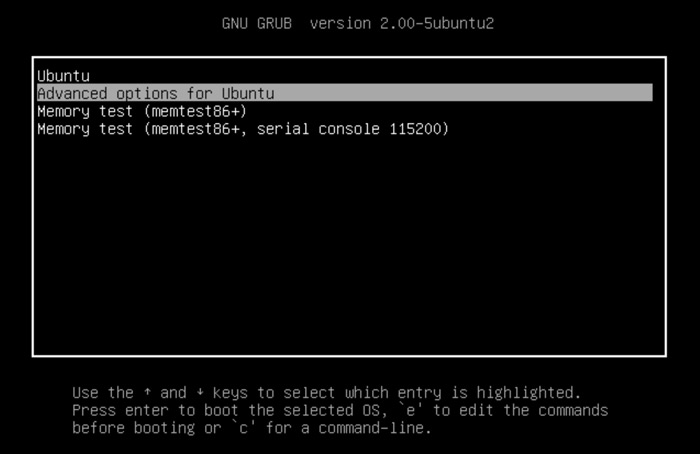
\includegraphics[width=11cm]{grub}
	\caption{Primer GRUB prozora tokom paljenja kompjutera}
\end{figure}
\end{itemize}


\subsection{Kernel}
Kernel je najvažniji i najosnovniji deo svakog operativnog sistema. Kernel je zadužen da pokrene svaku komponentu potrebnu za korišćenje sistema, da služi kao posrednik u komunikaciji izmedju softvera i hardvera, i delova softvera medjusobno. Kernel je potreban tokom celog korišćenja računara, pa je stoga neophodno da on bude što manji i što efikasniji.\\
Osnovi delove kernel-a su obično:
\begin{itemize}
\item rasporednik - odredjuje kako će razni procesi koristiti snagu procesora.
\item supervizor - odobrava kontrolu kompjutera procesu koji je na redu.
\item rukovodilac zahteva - rukuje svim zahtevima upućenim kernel-u.
\item menadžer memorije - dodeljuje lokacije na memoriji procesima kernel-a.
\end{itemize}
Postji 4 glavne kategorije kernel-a:
\begin{itemize}
\item monolitski - obično se nadju kod Unix-sličnih operativnih sistema, Linux i FreeBSD su primeri. Oni sadrže sve osnove funkcije OS-a i drajvere potrebne za korišćenje hardvera kao hard diskova, grafičkih kartica, printera, itd. Moderni monolitski kernel-i imaju opciju da odrede koji moduli kernel-a će se koristiti, time smanjujući količinu koda kernel-a.
\item microkernel - imaju samo minimalan broj usluga kao menadžer memorije, sistem za komunikaciju izmedju procesa i menadžer procesa. Sve ostale funkcije su implementirane nezavisno od kernel-a. Primeri mikrokernel-a su GNU Herd, MINIX i Mac OS X.
\item hibridni - kompromis izmedju monolitskih i mikrokernel-a. Osimišljeni se pre nego što je otkriveno da su mikrokernel-i daleko efikasniji od hibridnih.\\
Eksperimentiše se sa exokernel-ima. Glavna razlika izmedju njih i ostalih vrsta kernel-a je što se jedino bave zaštitom harvera umesto menadžmentom hardvera. Ovim pristupom exokernel-i omogućuje programerima da bolje odrede kako najefikasnije da koriste raspoloživ hardver.
\end{itemize}
\newpage
\subsection{Daemoni}
Daemon je program na Linux sistemima koji radi u pozadini, bez direktne kontrole korisnika. Oni obično služe da odgovaraju na zahteve drugih kompjutera na mreži, ali takodje, da reaguju na softverske i hardverske promene na samom kompjuteru.\\
Na primer, na daemon-e mogu da utiču odredjeno vreme ili datum, stvaranje fajla u specifičnom folderu, zahtev napravljen preko interneta, itd.
Daemon-i se vode u sistemu kao potprocesi ``init'' procesa, što je prvi proces koji se pokreće sa kompjuterom.\\
Na većini novih Linux sistema, daemon-i se pale samo po potrebi i na zahtev jednog glavnog daemon-a - ``xinetd''.

\subsection{Shell}
Shell služi da obezbedi isključivo tekstualni ``interfejs'' za korisnika. Njegova primarna svrha je čita komande iz konzole i da ih pokrene.\\
Naziv ``shell'' ili ``ljuska'' se odnosi na to da je to spoljašnji sloj opertivnog sistema tj. shell je posrednik izmedju korisnika i unutrašnjih delova sistema. Osim za sa samo pokretanje programa, shell-ovi imaju sposobnost da usmeravaju \textit{output} jedne komande da bude korišćen kao \textit{input} druge komande - ``piping'' (prvo uvedeno još u UNIX-u) i takodje da služe kao programski jezik - sintaksa komandi može da se koristi za pisanje ``shell skripti''.\\
Postoje razni shell-ovi, od kojih je najpopularniji ``bash'' (Bourne-again shell),  koji je nadogradnja na ``sh'' (Bourne shell) - originalni UNIX shell.
\subsection{X window sistem}
X window sistem ili samo ``X'' je sistem za menadžment grafičkih interfejsa (GUIs) na Linux-u. \textit{Window sistem} je kolekcija softvera koja omogućava korisniku lakšu kontrolu nad stvaranjem prozora i drugih grafičkih elemenata na kompjuteru.\\
Važna karakteristika X-a je što je odvojen od opertivnog sistema, za razliku kod Windows-a i starijih verzija Mac sistema gde je window sistem bio sastavni deo operativog sistema. Na Linux-u, i bez window sistema, sistem može da se kontroliše kroz komandni interfejs (CLI).\\
Još jedna važna karakteristika X-a je što je on samo mehanizam za korisnički interfejs, bez da odredjuje kakav će on biti. Ovo daje korisniku slobodu da sam odredi kakav interfejs želi, za raliku od drugih opertivnih sistema gde je unapred odredjeno kako će interfejs izgledati, sa minimalno prostora za promenu. Takodje je važno napomenuti da korisnik nije u kontaktu sa X-om. Aplikacije su same zadužene za svoje ponašanje i izgled, X služi samo da ih prikaže. Na početku je predstavljalo problem što je svaki program izgledao drugačije, jer je svaki dolazio sa svojim sopstevnim podešavanjima. Ovaj problem je rešen sa desktop okruženjima.\\
\begin{figure}[H]
	\centering
	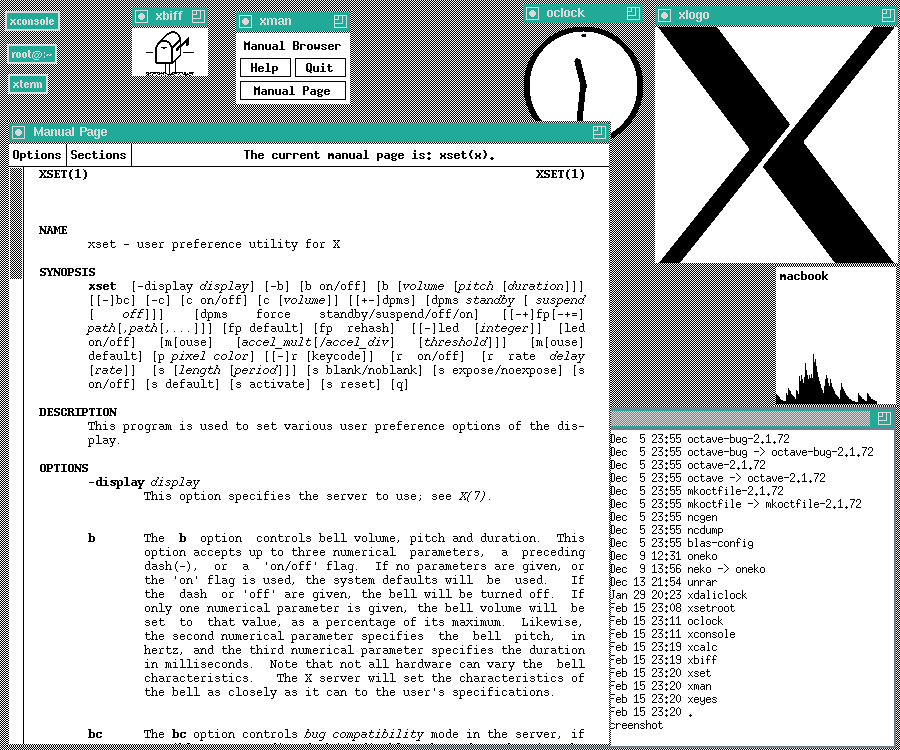
\includegraphics[width=11cm]{x}
	\caption{X u svojim ranim fazama, kasne 80-te i rane 90-te}
\end{figure}
\subsection{Desktop okruženje}
Desktop okruženje je skup softvera i drajvera koji rade na već postojećem sistemu sa gorenavedenim komponentama i služe da korisniku pruže što jednostavnije korišćenje sistema. Najpopularnija desktop okruženja su GNOME, KDE, Xfce, LXDE.
\begin{figure}[h]
	\centering
    \subfloat[GNOME desktop okruženje]{{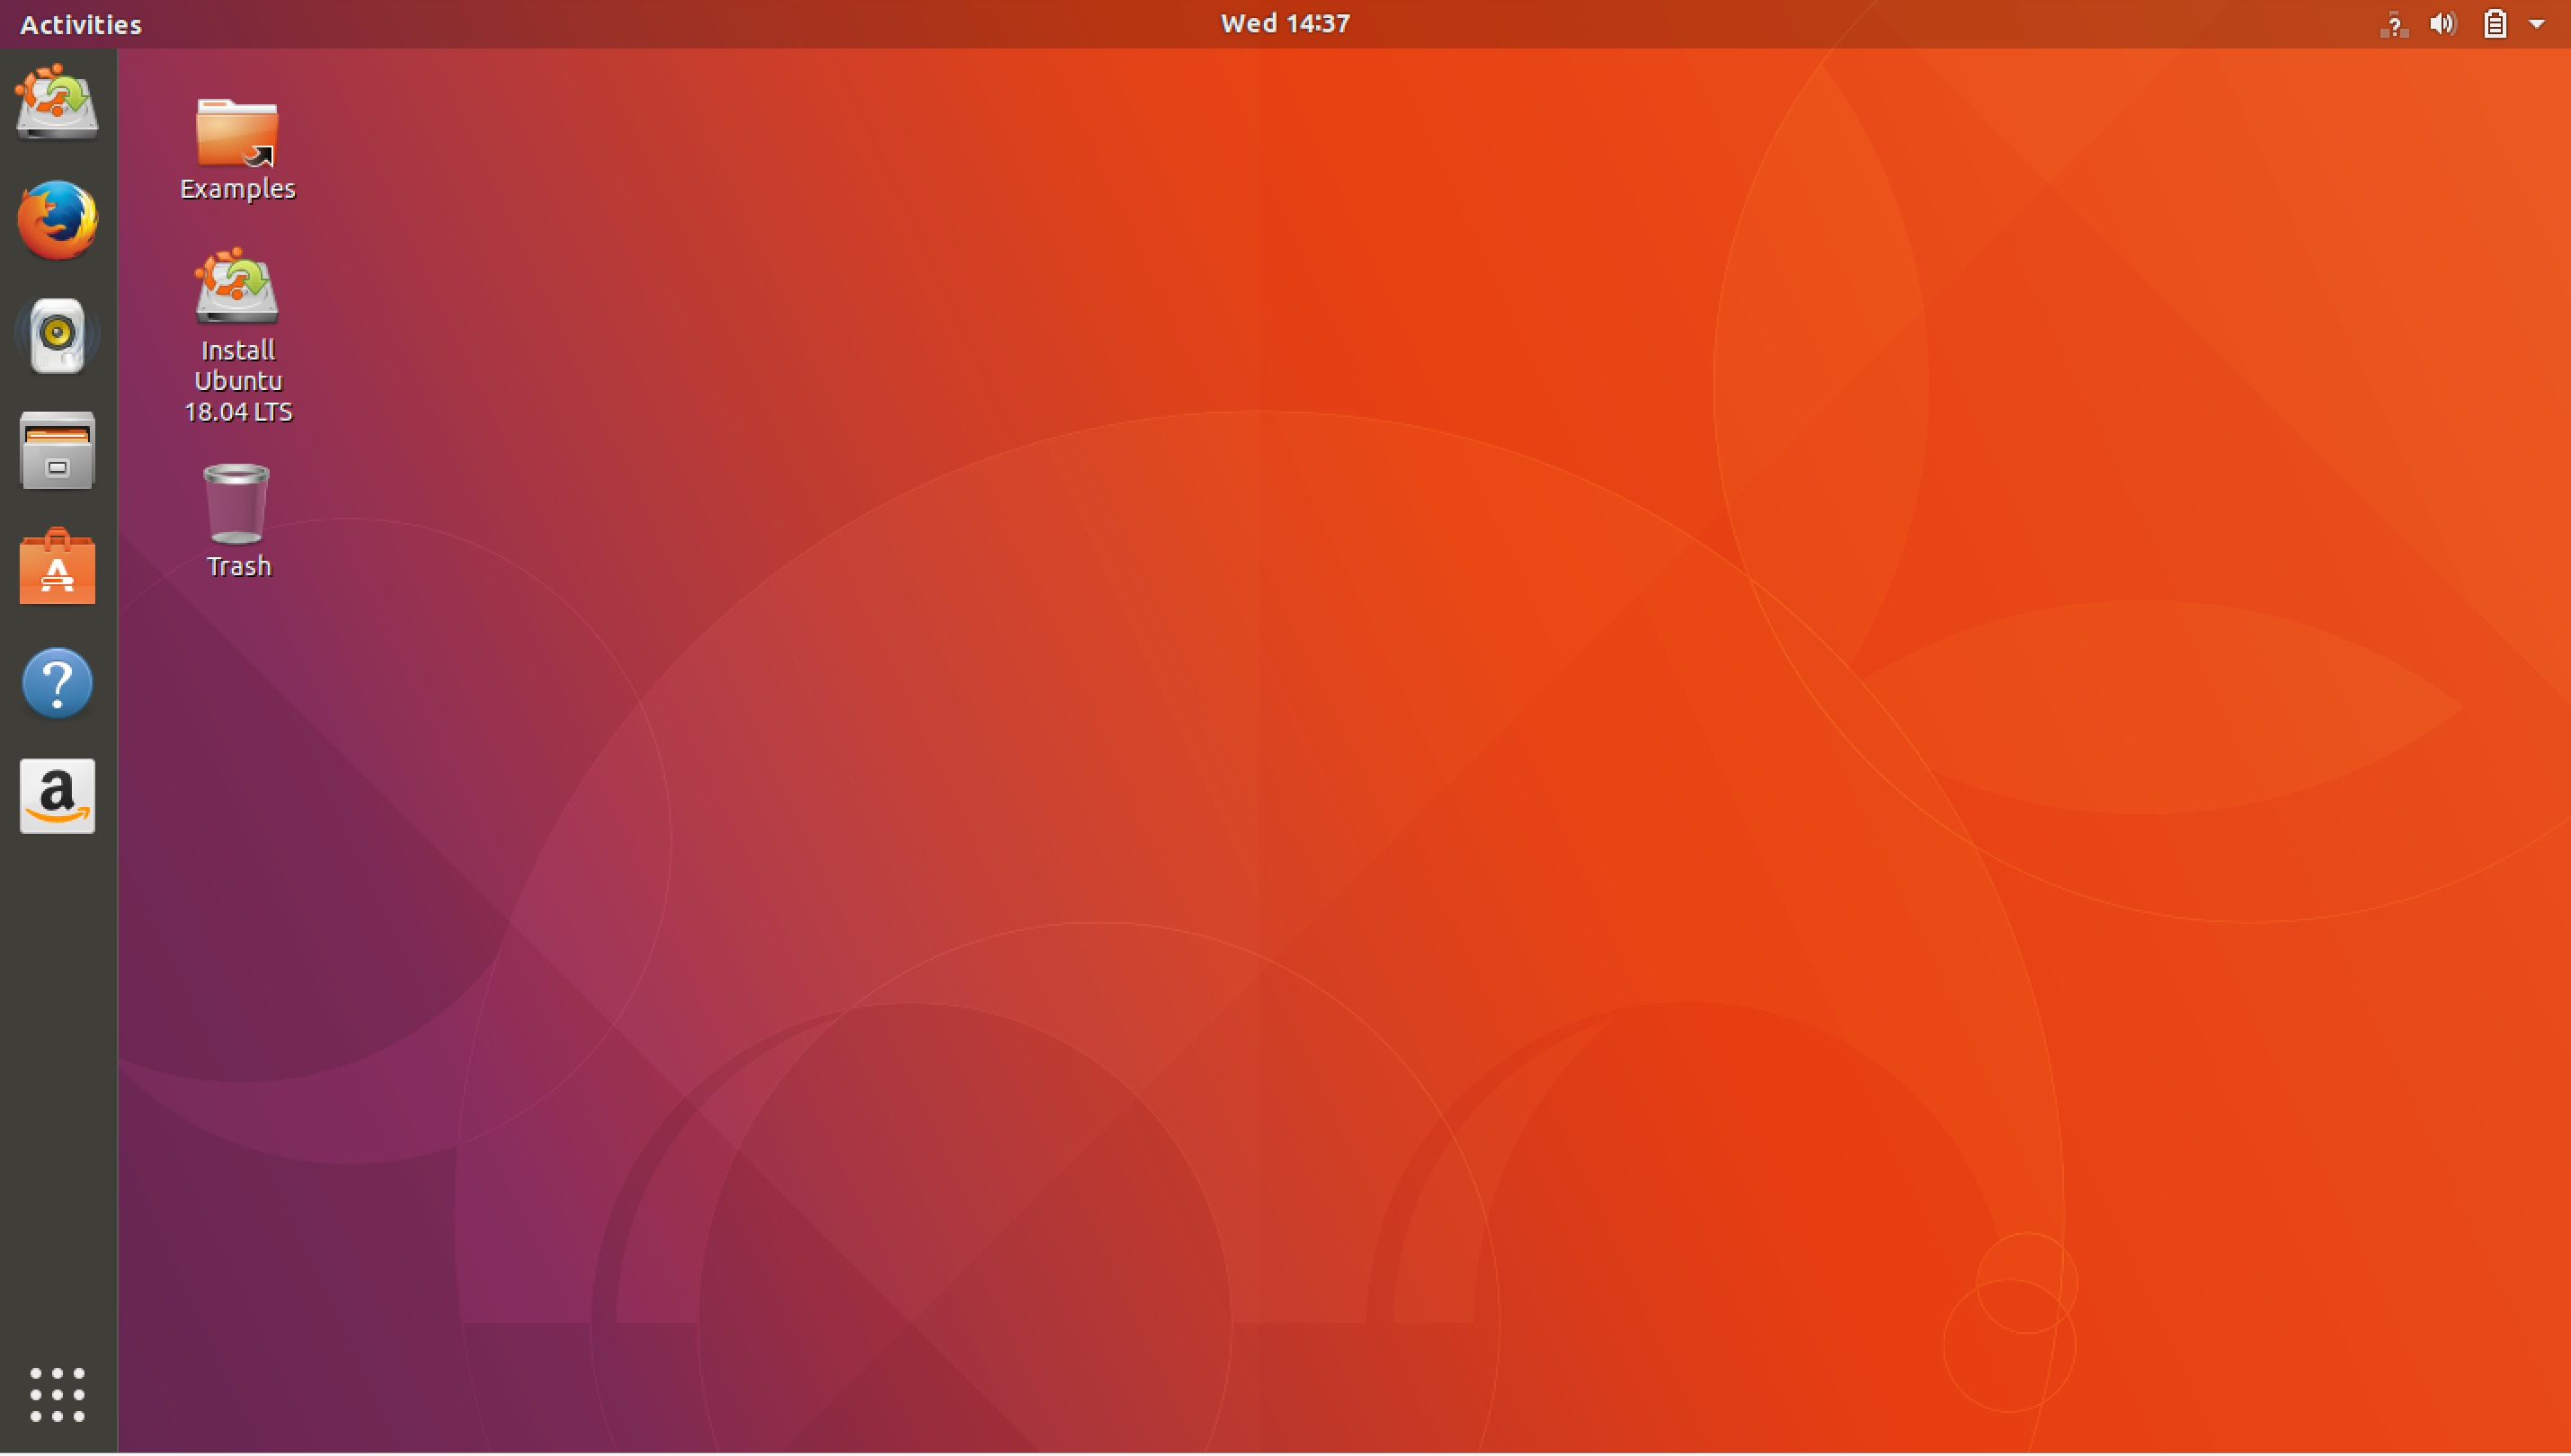
\includegraphics[height=6cm,width=7cm]{gnome} }}
    \qquad
    \subfloat[KDE desktop okruženje]{{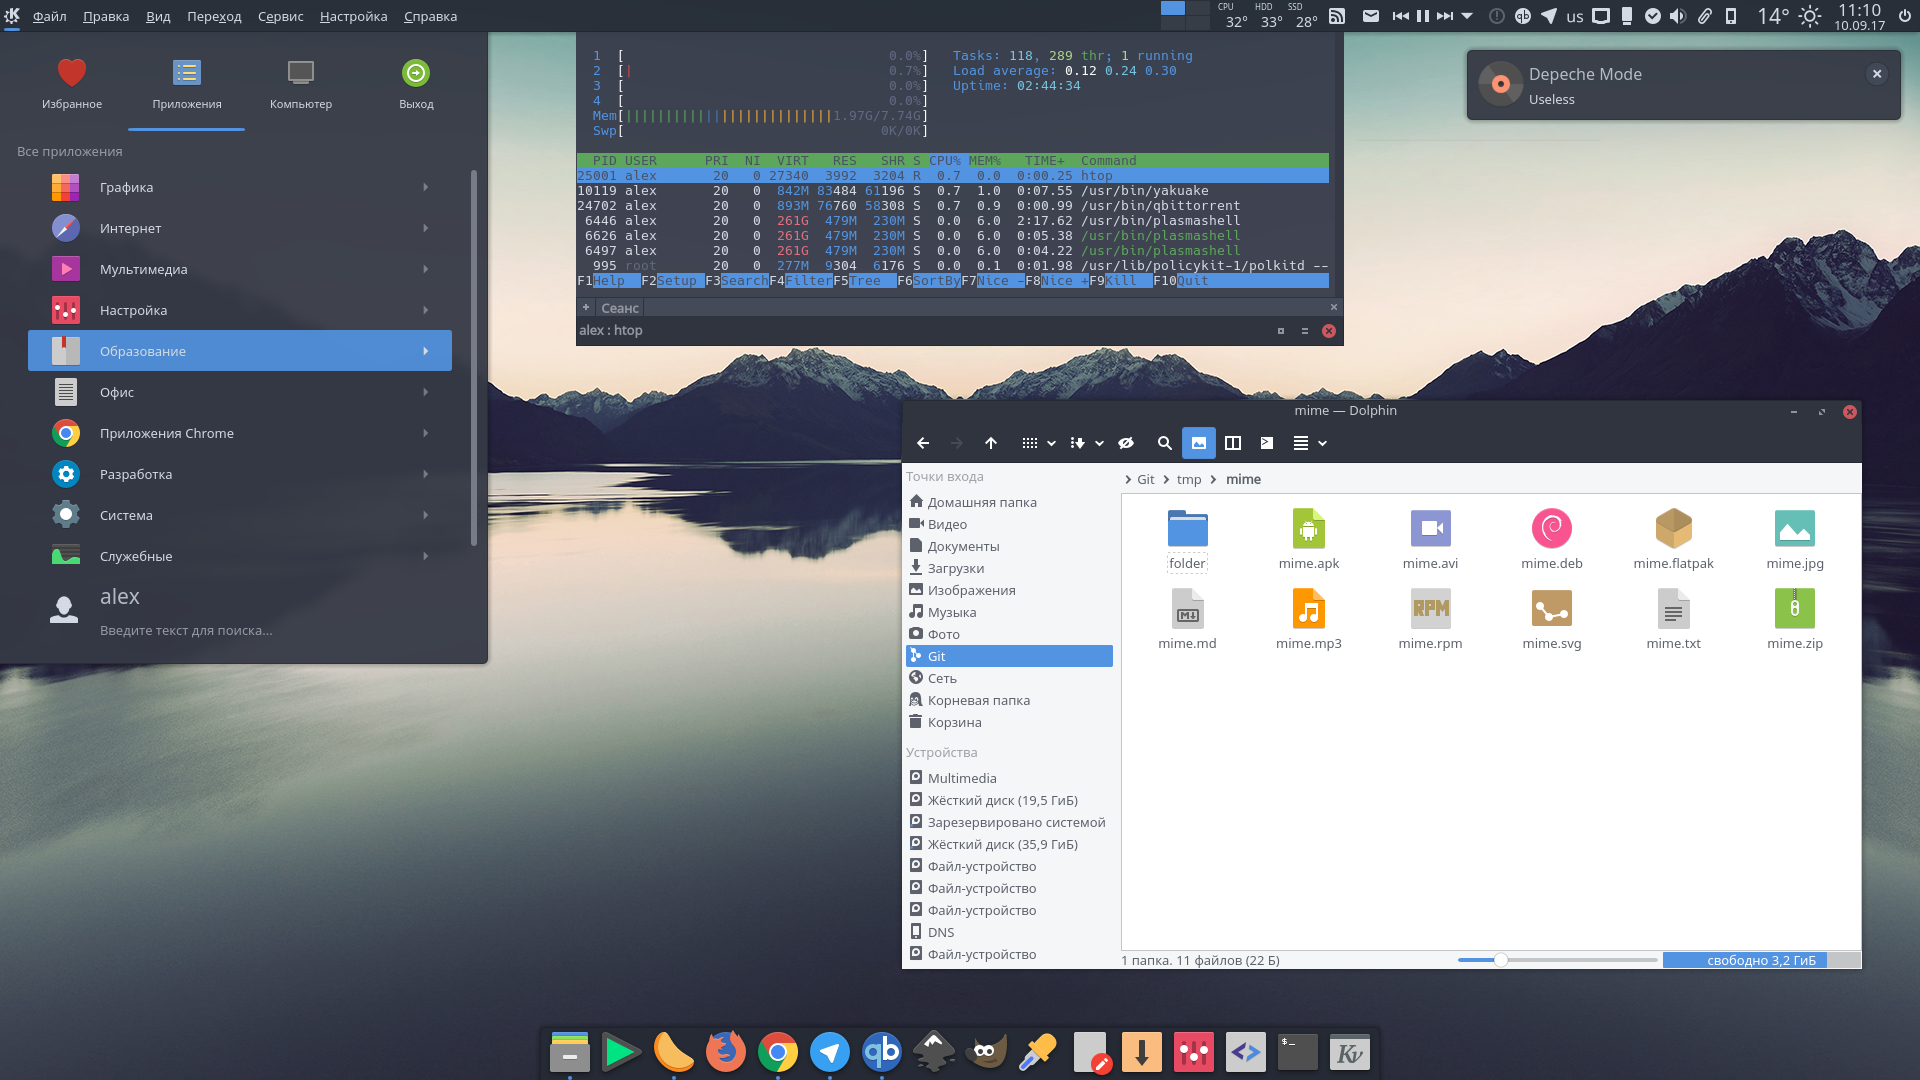
\includegraphics[height=6cm,width=7cm]{kde} }}
\end{figure}
\begin{figure}[h]
	\centering
    \subfloat[XFCE desktop okruženje]{{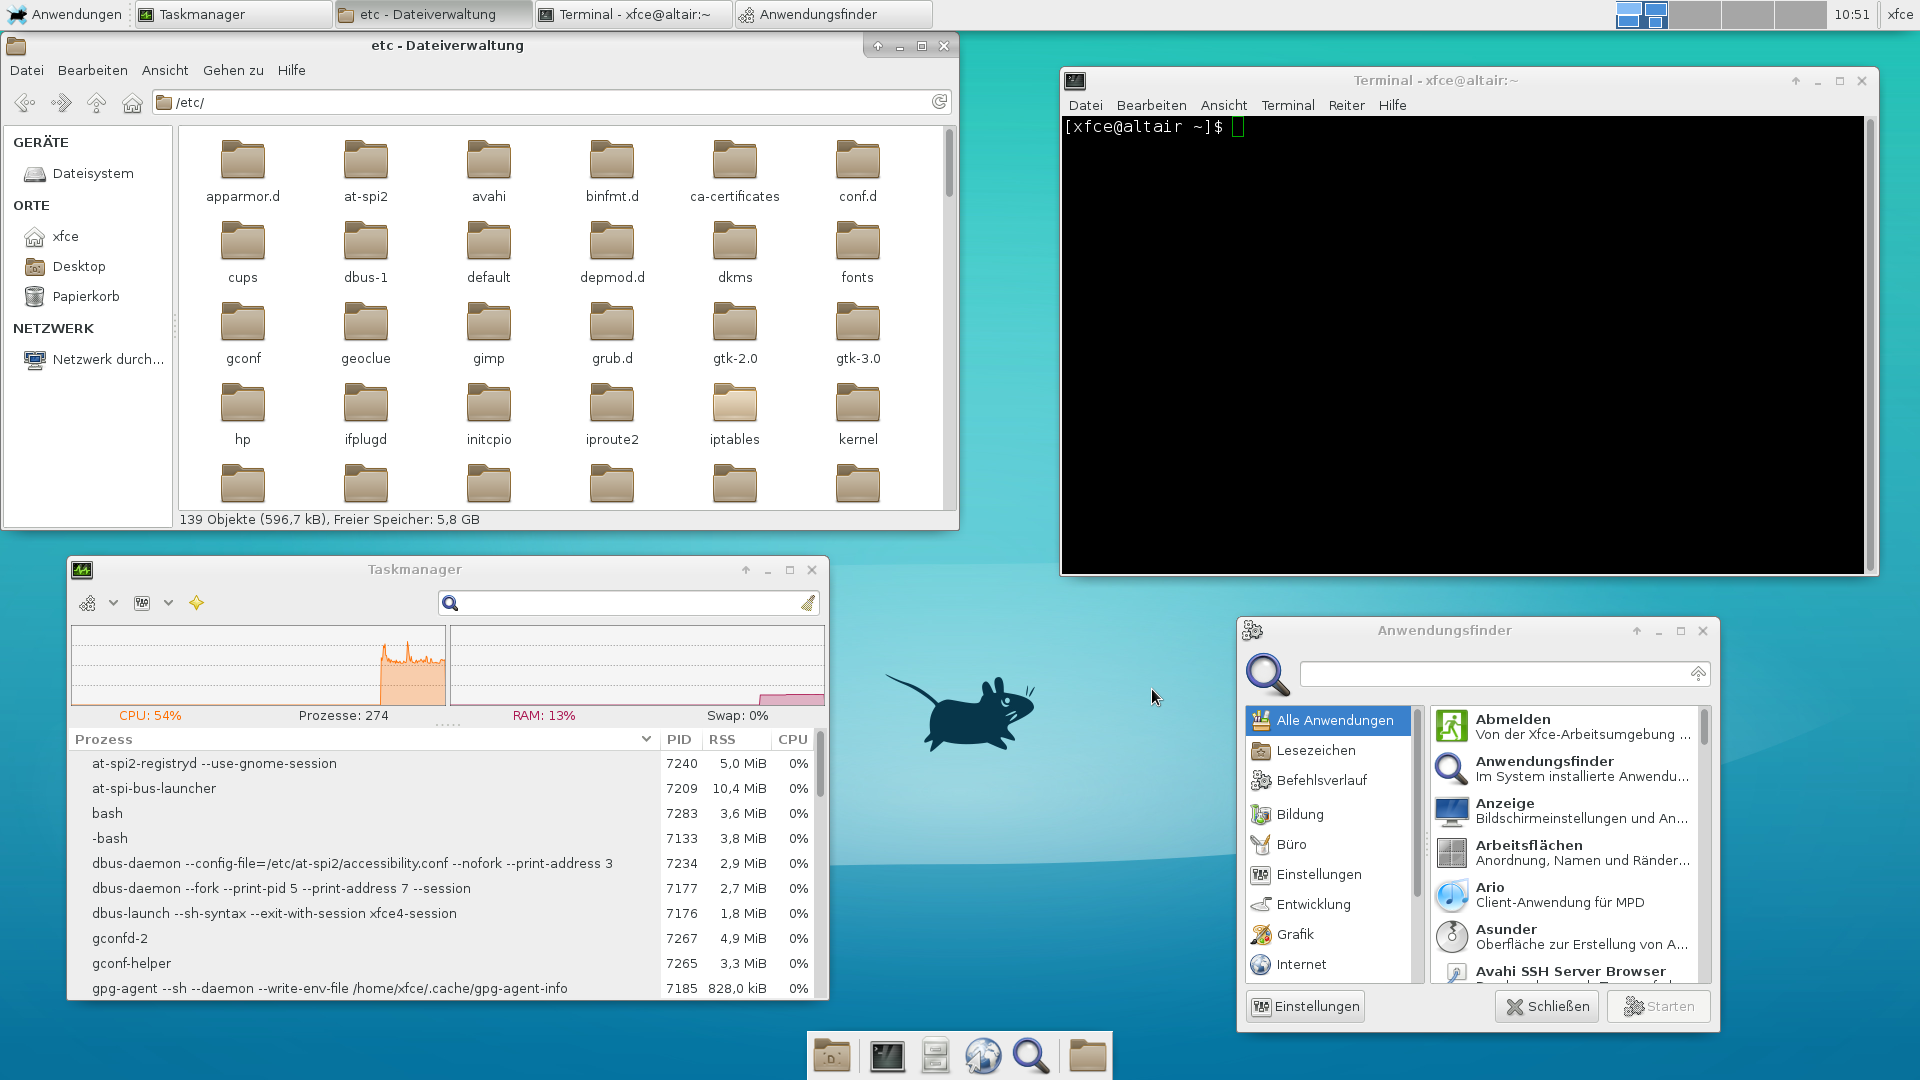
\includegraphics[height=6cm,width=7cm]{xfce} }}
    \qquad
    \subfloat[LXDE desktop okruženje]{{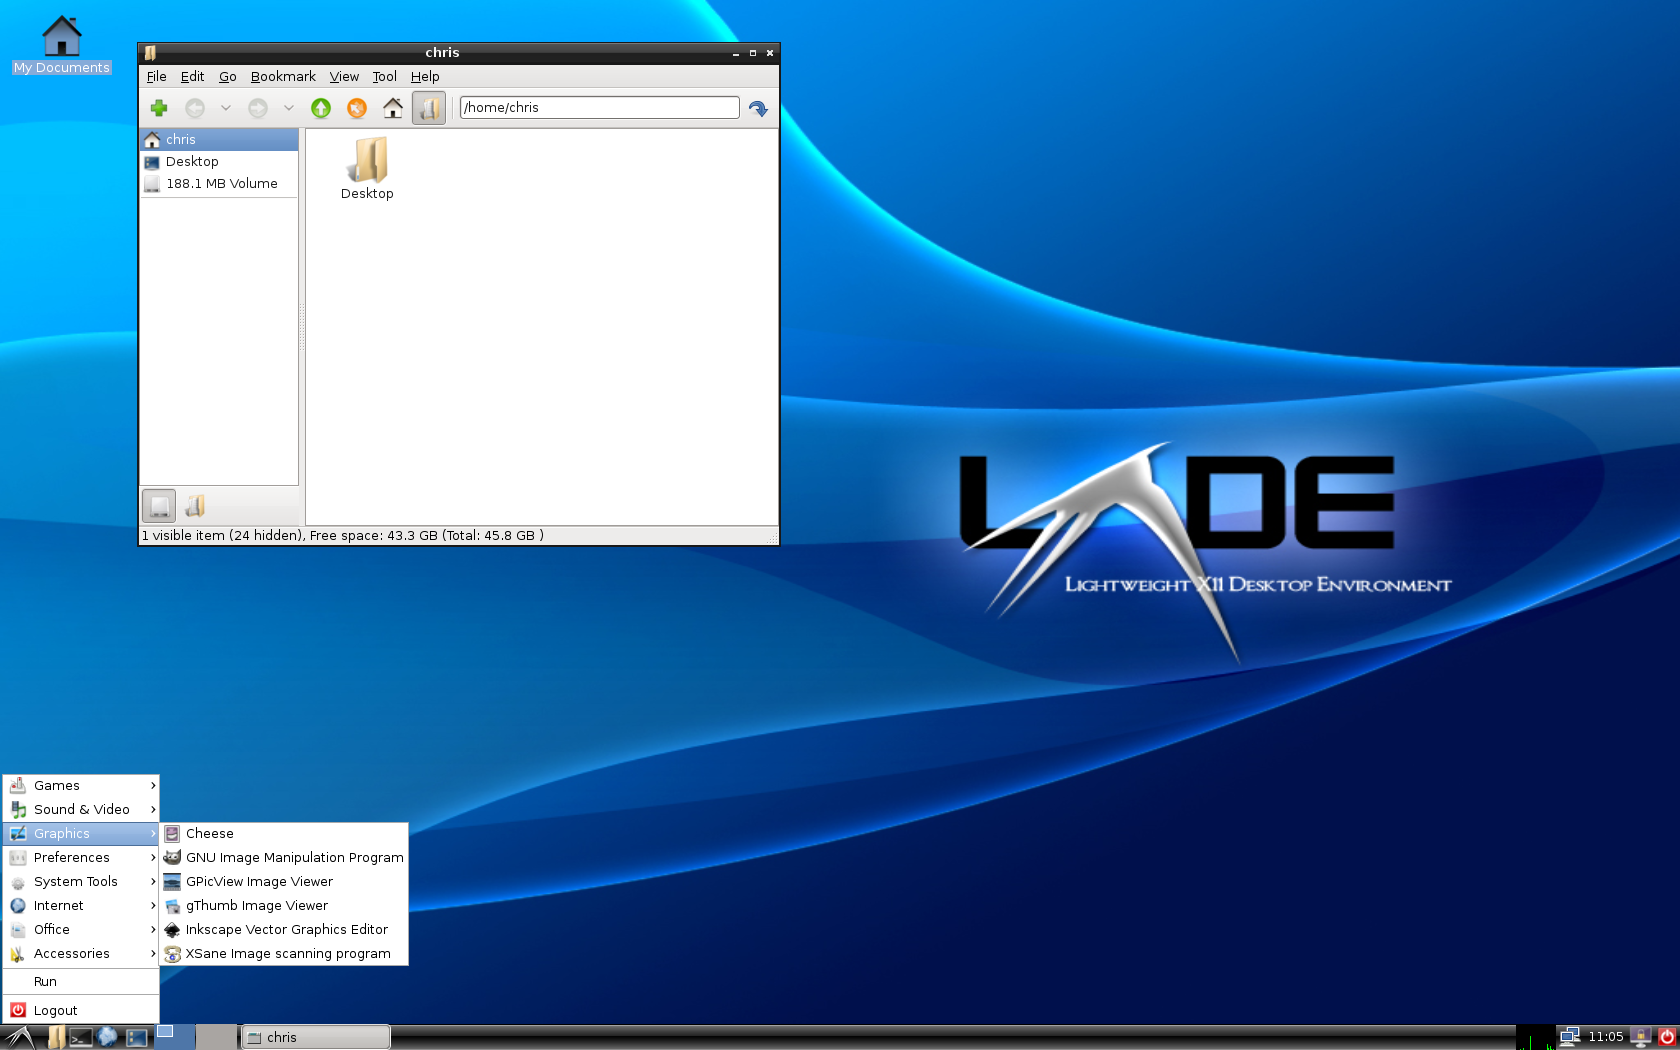
\includegraphics[height=6cm,width=7cm]{lxde} }}
\end{figure}